\section{Proba--V preprocessing}
As stated before, it was decided to use Proba-V as the augmentation training dataset.
As a preprocessing step, before training the high and low--resolution images should be aligned.
Some architectures, like the \textit{HighRes--net} feature deep learning based built--in mechanisms for image registration.
However, for training a simple image--downscaling augmentation network, a more traditional approach to image alignement can be implemented.
The preparation of dataset requires to turn the single high--resolution and multiple low--resolution imageset into high and low--res pairs.
This can be done by multiplying high--resolution images and aligning each copy with the corresponding low--resolution one.
Registering shift between images can be done using \textit{phase--correlation} \cite{guizar-2008-registration}.
This method utilizes two--dimensional \textit{Fourier transform}.
To register sub--pixel translations, images can be upscaled before applying the algorithm.
Since images to be aligned in Proba are of different resolution, they should be resized to common shape before registration.
It was decided to perform registration in the high--resolution image domain.
Shifting images will create blank columns and rows on their borders, which were removed by cropping the images.
It is known that low--resolution images in Proba have sub--pixel dislocation, for this reason they should be cropped with one pixel border.
High--resolution images are three times larger, consequently, a margin of three pixels should be removed from them.
After this step of preprocessing high--res images are 378 by 378 pixels and low--resolution photos are 126 by 126 pixels.
It is valuable to visualize the effects of the registration process to ensure its correctness.
Because Proba images have single depth dimension, they can be visualized as different color channels.
This technique is utilized in the figure \ref{fig:proba-registration}, where red and blue channels contain two pictures that are to be registered.
If the pictures are aligned perfectly, the image should be yellow because red and blue channels overlay perfectly.
The more unaligned the pictures are the more red and blue is visible in the picture, which is most visible at distinct edges.
The visualization proves that the phase--correlation based registration is suitable for the Proba--V dataset---after registration the picture becomes more yellow and the unaligned edges are less visible.
\begin{figure}
    \begin{subfigure}{0.45\textwidth}
        \centering
        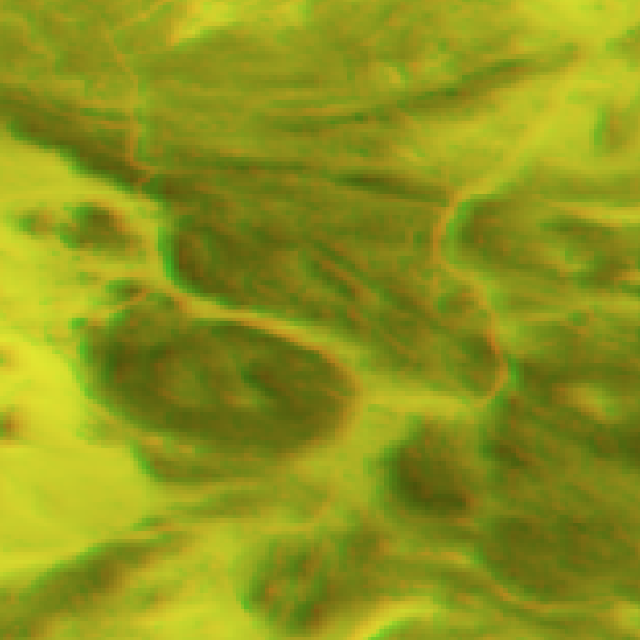
\includegraphics[width=\textwidth]{proba_unregistered}
        \caption{Proba--V images overlay before registration}
    \end{subfigure}
    \hfill
    \begin{subfigure}{0.45\textwidth}
        \centering
        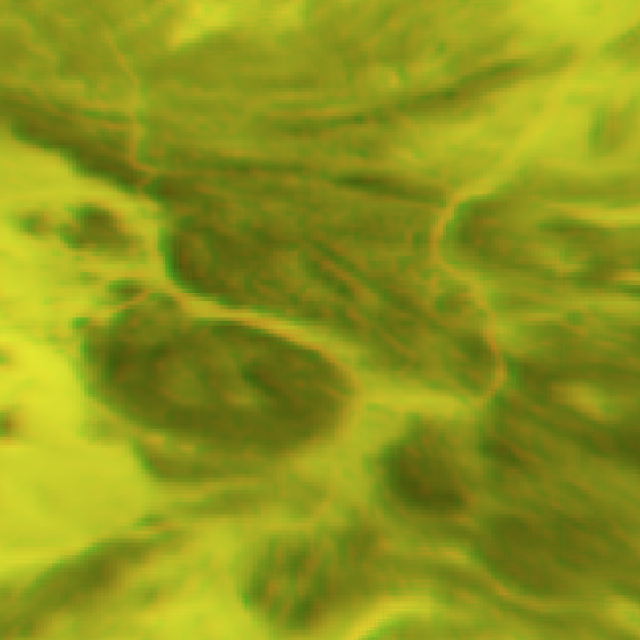
\includegraphics[width=\textwidth]{proba_registered}
        \caption{Proba--V images overlay after registration}
    \end{subfigure}
    \caption{Sample image pair from \textit{Proba--V NIR train dataset}}
    \label{fig:proba-registration}
\end{figure}

Photos in the Proba--V dataset are saved as sixteen-bit images; however, only fourteen--bit values are utilized.
It should be noted, to scale the images properly.
Using Proba--V dataset with real--life high and low--resolution images poses an additional challange.
As stated, the images contained in the dataset are taken at different moments, thus they differ in exposure and contrast.
Images in high and low--res pairs differ in brightness, both at the level of local details and global average values.
Distributions of image exposure in the dataset are presented in the figures \ref{fig:exposure-dist-red} and \ref{fig:exposure-dist-red} for RED and NIR subsets.
\begin{figure}
        \centering
         \begin{tikzpicture}
		 \begin{axis}[width=\textwidth, height=4cm, grid=major, grid style={dashed}, xmin=0, xmax=0.9, ytick={1, 2}, yticklabels={High--res, Low--res}]
		      \addplot+ [boxplot prepared={draw position=1,
		      							   average=0.30,
		                                   median=0.28,
		                                   lower whisker=0.1,
		                                   upper whisker=0.60,
		                                   upper quartile=0.37, 
		                                   lower quartile=0.21}] 
		                                   coordinates {(1,0.78)(1,0.66)};
		       \addplot+ [boxplot prepared={draw position=2,
		      							   average=0.31,
		                                   median=0.28,
		                                   lower whisker=0.10,
		                                   upper whisker=0.63,
		                                   upper quartile=0.38, 
		                                   lower quartile=0.21}] 
		                                   coordinates {(2,0.83)(2,0.69)};
		  \end{axis}
		  \end{tikzpicture}
    \caption{Exposure distributions in the RED Proba--V dataset}
    \label{fig:exposure-dist-red}
\end{figure}
\begin{figure}
        \centering
                 \begin{tikzpicture}
		 \begin{axis}[width=\textwidth, height=4.5cm, grid=major, grid style={dashed}, xmin=0.2, xmax=1, ytick={1, 2}, yticklabels={High--res, Low--res}]
		      \addplot+ [boxplot prepared={draw position=1,
		      							   average=0.47,
		                                   median=0.44,
		                                   lower whisker=0.31,
		                                   upper whisker=0.65,
		                                   upper quartile=0.52, 
		                                   lower quartile=0.40}] 
		                                   coordinates {(1,0.93)(1,0.85)(1,0.78)};
		       \addplot+ [boxplot prepared={draw position=2,
		      							   average=0.48,
		                                   median=0.45,
		                                   lower whisker=0.27,
		                                   upper whisker=0.68,
		                                   upper quartile=0.54, 
		                                   lower quartile=0.40}]
		                                   coordinates {(2,0.90)(2,0.89)(2,0.82)};
		  \end{axis}
		  \end{tikzpicture}
    \caption{Exposure distributions in the RED Proba--V dataset}
    \label{fig:exposure-dist-red}
\end{figure}


Having a dataset with high and low--resolution images of different brightness and contrast can be an obstacle for learning a neural network.
For this reason, \textit{histogram equalization} was applied to the learning data.
This technique enhances image contrast and evens the histogram of pixel values.
After equalization, the cumulative distribution of brightness is close to linear.

As noted previously, Proba--V includes binary masks denoting areas of images that are suitable for training.
Some images include noticeable large areas of unusable pixels.
For this reason, nine images with the least the percentage of invalid pixels were chosen per scene as training data.
This excludes incorrect data from the training set.  

\section{Augmentation network architectures}
The augmentation network is to perform a rather simple task of reducing the size of input pictures.
Three architectures that perform this task have been created, they are presented with an increasing complexity.

\subsection{Simple fully--convolutional network}
The most simplistic approach to shrinking images with deep learning is to build a basic, fully convolutional network.
The most simplistic implementation of this idea uses three convolutional layers with kernels of size three by three.
The midmost convolution slides the filter window with a stride of three to decrease the size of input by three times.
The last convolutional layer features one filter to reduce the output depth to a single channel.
\textit{ReLU} activation function was used for each applicable layer.
A precise description of the architecture is presented in the table \ref{tab:simple-conv-arch}.
\begin{table}
    \centering
    \caption{Simple fully--convolutional network architecture for data augmentation}
    \label{tab:simple-conv-arch}
    \begin{tabular}{ccc}
        \toprule
        Layer type & Output Shape & Number of parameters \\
        \midrule
        $ Input $      & 378, 378, 1  & 0                    \\
        $ Conv2D(filters=64, stride=1) $ & 378, 378, 64 & 640 \\
        $ ReLu $ & 378, 378, 64 & 0 \\
        $ Conv2D(filters=64, stride=3) $ & 126, 126, 64 & 36928 \\
        $ ReLU $ & 126, 126, 64 & 0 \\
        $ Conv2D(filters=1, stride=1) $ & 126, 126, 1 & 577 \\
        $ Sigmoid $ & 166, 126, 1 & 0 \\
        \bottomrule
    \end{tabular}
\end{table}

\subsection{Fully--convolutional encoder--decoder network}
The more complex architecture that can be applied is based on the previously mentioned encoder--decoder network scheme.
It is one of the most popular image--to--image neural network architectures.
The encoder shrinks the image by a factor of six instead of three.
Then the image is upscaled two times.
In result, the output image is overall three times smaller; however, it has been processed by more convolutional layers than in the simple convolutional network.

There are various ways to upscale the image during the decoding process.
The main ones are traditional upscaling and a \textit{transposed convolution} (sometimes called \textit{deconvolution}).
The later performs a convolution and then transposes the output, which makes the spatial dimension grow in size.
However, the transposed convolution layers can produce visible checkerboard artifacts on the image \cite{odena-2016-deconvolution}.
For this reason, the simpler layer architecture based on upscaling was chosen.
Like the simple architecture, the encoder--decoder features a convolution with a single filter at the end.
The detailed description of the network is shown in the table \ref{tab:autoencoder-arch}.
\begin{table}
    \centering
    \caption{Encoder--decoder network architecture for data augmentation}
    \label{tab:autoencoder-arch}
    \begin{tabular}{ccc}
        \toprule
        Layer type & Output Shape & Number of parameters \\
        \midrule
        $ Input $      & 378, 378, 1  & 0                    \\
        $ Conv2D(filters=64, stride=1) $ & 378, 378, 64 & 640 \\
        $ ReLU $ & 378, 378, 64 & 0 \\
        $ Conv2D(filters=64, stride=3) $ & 126, 126, 64 & 36928 \\
        $ ReLU $ & 378, 378, 64 & 0 \\
        $ Conv2D(filters=64, stride=2) $ & 126, 126, 64 & 36928 \\
        $ ReLU $ & 378, 378, 64 & 0 \\
        $ UpSampling2D(stride=2) $ & 126, 126, 64 & 0 \\
        $ Conv2D(filters=1, stride=1) $ & 126, 126, 1 & 577 \\
        $ Sigmoid $ & 166, 126, 1 & 0 \\
        \bottomrule
    \end{tabular}
\end{table}

\subsection{Generative adversarial network}
In recent years, a new approach to training generative neural networks has emerged.
The traditional supervised learning described in the previous sections consists in providing the network with an input and comparing the generated output with a ground truth to compute loss.
The \textsc{gan}---\textit{generative adversarial network} approach requires creating two networks, a \textit{generator} and \textit{discriminator} \cite{goodfellow-2014-gans}.
The former is tasked with generating data, while the latter learns to differentiate images created by the generator from real ones.
In the \textsc{gan} scheme the discriminator learns like a traditional binary classifier---it is provided with real and generated images, which are labeled accordingly.
Then discriminator loss is computed using standard classification metrics like \textit{binary cross--entropy}.
However, the generator learns in a more unique way; it creates an output image that is fed into a discriminator.
The generator loss is calculated depending on how well it produces data that may be classified as \textit{real} by a discriminator.
If the generated image is recognized as a \textit{fake} one, it receives a big penalty in the form of a large loss.

\textsc{Gan}s can have many variations, the most common variant utilizes unsupervised or semi--supervised data generation.
A great advantage of this kind of network is the ability to create images without direct input.
Usually a \textsc{gan} generator creates output from random values.
These values are randomly initiated inside proper \textit{latent space}.
However, adversarial networks can also work in fully--supervised way.
In this work a \textsc{gan} is proposed that transforms high--resolution images to low--resolution, with loss calculated in regard to the discriminator's judgements.
Such networks are often called picture--to--picture \textsc{gan}s.
An algorithm for training such a network is provided in the pseudocode listing \ref{alg:gan-training}.
One further optimization can be applied to \textsc{gan}---usually better results are achieved if small noise is applied to the labels.
\begin{algorithm}
\caption{\textsc{Gan} training flow}
\label{alg:gan-training}
\begin{algorithmic}
	\REQUIRE{$ x $, $ y_{gt} $}
	\STATE $ y_{fake} = generator(x) $
	\STATE $ y_{pred} = discriminator(cat(y_{fake}, y_{gt})) $
	\STATE $ loss_d = lossfn_d(y_{pred}, cat(\mathds{O}, \mathds{1})) $
	\STATE $ optimze_d(loss_d) $
	\STATE $ freeze\_learning(discriminator) $
	\STATE $ y_{pred} = discriminator(generator(x)) $
	\STATE $ loss_g = lossfn_g(y_{pred}, \mathds{1}) $
	\COMMENT{Notice the misleading labels matrix}
	\STATE $ optimize_g(loss_g) $
\end{algorithmic}
\end{algorithm}
The fitting process of a \textsc{gan} network can also be visualized in the form of a graph, as presented in the figure \ref{fig:gan-training}.
\begin{figure}
    \centering
    \documentclass[tikz]{standalone}
\usepackage[utf8]{inputenc}

\usetikzlibrary{positioning}
\usetikzlibrary{shapes}
\usetikzlibrary{calc}

\begin{document}
	
\tikzset{arrow/.style={-stealth}}

\begin{tikzpicture}[ampersand replacement=\&]
   	\node[text width=0.25cm] at (-2.5,0) (X) {$ \mathbf x $};		 
    \node[rectangle, rounded corners, draw, fill=blue!20, minimum height=1cm] at (0,0) (G) {\textsc{Generator}};	
    \node[rectangle, rounded corners, draw, minimum height=1cm] at (3,0) (S1) {\textsc{Sample}};
    
    \node[text width=0.5cm] at (0.75,3) (Y) {$ \mathbf y_{gt} $};		 
    \node[rectangle, rounded corners, draw, minimum height=1cm] at (3,3) (S2) {\textsc{Sample}};
    
    \node[rectangle, rounded corners, draw, fill=blue!20, minimum height=1cm] at (6,1.5) (D) {\textsc{Discriminator}};
    
    \node[text width=2cm] at (10,1.5) (O) {\textsc{Real/Fake Prediction}};
     
    \path[arrow] (X) edge (G)
    (G) edge (S1)
    (S1) edge (D.south west)
    (Y) edge (S2)
    (S2) edge (D.north west)  
    (D) edge (O)
    ;
\end{tikzpicture}

\end{document}
    \caption{Schematic of \textsc{gan} network inner--workings}
    \label{fig:gan-training}
\end{figure}

The discriminator architecture reassembles a common binary classifier with convolutional and polling layers.
A \textit{leaky ReLu (rectified linear unit)} was used as an activation function.
After applying a series of convolutions, the image is flattened and then densely connected.
A common problem encountered during \textsc{gan} networks is too rapid fitting of the discriminator.
Because it is tasked with a much simpler task than the generator, the discriminator tends to overwhelm its opponent.
For this reason, the discriminator is often handicapped in a way.
In this case it is missing a large densely connected layer after flatten operation, which would be otherwise typically used in a binary classifier.
Moreover, a stride of size two is combined with a pooling operation to perform more rapid spatial shrinking of the image and put the discriminator at a disadvantage.
Furthermore, a dropout layer was used right before the end of the network.
This kind of layer drops a part of data to prevent overfitting (and also slow down the learning process).
A detailed description of the discriminator part of \textsc{gan} can be found in the table \ref{tab:discriminator-arch}.
\begin{table}
    \centering
    \caption{\textsc{Gan} architecture discriminator for data augmentation}
    \label{tab:discriminator-arch}
    \begin{tabular}{ccc}
        \toprule
        Layer type & Output Shape & Number of parameters \\
        \midrule
        $ Input $      & 126, 126, 1  & 0                    \\
        $ Conv2D(filters=64, stride=2) $ & 63, 63, 64 & 640 \\
        $ LeakyReLU $ & 63, 63, 64 & 0 \\
        $ MaxPool2D(stride=2) $ & 31, 31, 64 & 0 \\
        $ Conv2D(filters=64, stride=2) $ & 16, 16, 64 & 36928 \\
        $ LeakyReLU $ & 16, 16, 64 & 0 \\
        $ MaxPool2D(stride=2) $ & 8, 8, 64 & 0 \\
        $ Flatten $ & 4096 & 0 \\
        $ Dropout(rate=0.5) $ & 4096 & 0 \\
        $ Dense $ & 1 & 4097 \\
        $ Sigmoid $ & 1 & 0 \\
        \bottomrule
    \end{tabular}
\end{table}
The generator is structured similarly to the previously presented fully--convolutional layers, as it performs a similar task.
The full architecture is the same as presented in the table \ref{tab:simple-conv-arch}.
\section{Training details}
The NIR subset of Proba--V dataset was used to train augmentation networks.
As mentioned before, Proba contains a set of binary masks designating areas of low--resolution images that may be invalid.
This has been taken into account in the two of the described networks---the simple--fully convolutional network and encoder--decoder.
If masks are used during training, the masked regions of low--res images do not participate in loss calculation.
This feature works only with per--pixel losses such as MAE and MSE.
Because SSIM works in a more structural way, it is not possible to remove some pixels from the evaluation when using this metric.

Both simple and encoder--decoder networks use \textit{ADAM (Adaptive Moment Estimation)} optimizer for gradient descent.
This kind of optimization algorithm combines advantages of \textit{momentum} technique and \textit{RMSprop}.
The momentum component uses a moving average of gradients from consecutive steps to update weights, instead of single gradient value, as traditional algorithms would use.
This modification helps the gradient descent to avoid slow downs on plateaus in the search space.
The RMSprop--alike part of ADAM is responsible for adaptive scaling of learning rate based on value of squared gradients.
Alongside ADAM optimizer, MSE was used as the loss function during the final training of the two simpler architectures.

To supervise the training process in an unbiased, way a validation data subset should be used.
Validation data is a part of the training set that doesn't take part in the gradient calculation, but is used to calculate loss and metrics every epoch.
This way the ongoing training can be evaluated on the data that is not directly used for the fitting process.
It is important to create the validation subset out of the training data, not the test dataset.
If the test data was used for validation, a data leak from the evaluation step to the training would occur.
In the training process of all models 20\% of the training dataset was used for the validation.
Both of the simpler architectures utilize \textit{early stopping} mechanism.
This technique stops training after a designated number of epochs without an improvement in the validation loss value.
Early stopping helps to avoid overfitting and provides a more rational stop condition than training for an arbitrary number of epochs.
Training history of the simple convolutional and the encoder--decoder network is presented in the figure \ref{fig:simple-encoder-decoder-train-hist}.
The subfigures show the simultaneous decrease of training and validation loss.
The decreasing loss curves reassemble an exponential decay function, which is a sign of proper training.
\begin{sidewaysfigure}
    \begin{subfigure}{0.5\textwidth}
    \hfill
        \centering
        \begin{tikzpicture}
			\begin{axis}[grid=major, grid style={dashed}, xlabel=Epoch, ylabel=Loss]
			\addlegendentry{Simple convolutional}
			\addplot+[mark=none] table [x=step, y=value, col sep=comma] {data/simple_conv-dvc-21-07-04-04_47_26-train_epoch_loss.csv};
			\addlegendentry{Encoder--decoder}
			\addplot+[mark=none] table [x=step, y=value, col sep=comma] {data/autoencoder-dvc-21-07-04-05_26_47-train_epoch_loss.csv};
			\end{axis}
		\end{tikzpicture}
        \caption{Training loss history}
    \end{subfigure}
    \hfill
    \begin{subfigure}{0.5\textwidth}
        \centering
        \begin{tikzpicture}
			\begin{axis}[grid=major, grid style={dashed}, xlabel=Epoch, ylabel=Loss]
			\addlegendentry{Simple convolutional}
			\addplot+[mark=none] table [x=step, y=value, col sep=comma] {data/simple_loss-dvc-21-07-04-04_47_26-validation_epoch_loss.csv};
			\addlegendentry{Encoder--decoder}
			\addplot+[mark=none] table [x=step, y=value, col sep=comma] {data/autoencoder-dvc-21-07-04-05_26_47-validation_epoch_loss.csv};
			\end{axis}
		\end{tikzpicture}
        \caption{Validation loss history}
    \end{subfigure}
    \hfill
    \caption{Training history of the simple convolutional and encoder--decoder netowrks}
    \label{fig:simple-encoder-decoder-train-hist}
\end{sidewaysfigure}

Training a \textsc{gan} can pose a significant challenge when stopping condition is taken into consideration.
More ordinary networks utilize early stopping mechanism on the validation dataset to limit the number of training epochs, as it was described previously.
When training \textsc{gan}, it is less obvious what should be used as a metric during validation.
The losses calculated during training do not explicitly express the quality of the outcome.
The generator loss indicates how well it performs relatively to the discriminator's ability to differentiate real and generated images.
This doesn't necessarily mean that the generator outputs high quality images.
It is better to apply a different metric on evaluation that omits the adversarial part of the network.
In this work, validation is based on calculating SSIM value of the generator output and ground truth.
This approach is not applicable to all \textsc{gan} networks because their training scenarios usually lack the possibility of comparing with any reference data.
Having an easily readable validation metric is beneficial for network evaluation; however, in this work it was not used to utilize early stopping with the \textsc{gan} network.
Adversarial networks tend to have more unstable and varied trainings than conventional networks.
Thus, it was decided to train the \textsc{gan} with a large fixed number of a hundred epochs.
History of training loss of discriminator and generator parts of a the GAN network are presented in the figure \ref{fig:gan-train-hist}.
The model from the epoch 94, with the highest SSIM validation score, was chosen as the best one and used to export augmented dataset in the further course of the work.
\begin{figure}
    \centering
    \begin{tikzpicture}
			\begin{axis}[width=0.75\linewidth, height=10cm, grid=major, grid style={dashed}, xlabel=Epoch, ylabel=Loss]
			\addlegendentry{Discriminator}
			\addplot+[mark=none] table [x=step, y=value, col sep=comma] {data/gan-dvc-21-07-04-05_55_06-train-epoch_d_loss.csv};
			\addlegendentry{Generator}
			\addplot+[mark=none] table [x=step, y=value, col sep=comma] {data/gan-dvc-21-07-04-05_55_06-train-epoch_g_loss.csv};
			\end{axis}
		\end{tikzpicture}
    \caption{Training history of GAN generator and discriminator subnetworks}
    \label{fig:gan-train-hist}
\end{figure}

The contents of the \textit{params.yaml} file used for training the augmentation networks are included in the appendix, in the chapter \ref{ch:appendix-params}.

\section{Intermediate results}
The experiment workflow assumes that an intermediate evaluation step can be performed between training augmentation and super--resolution networks.
The Proba--V test dataset can be used to test how well the low--resolution images are recreated by the neural networks.
It should be noted that the following results are an intermediate step to sanity--check if augmented pictures are reconstructed correctly.
At this step, the results do not guarantee the quality of super--resolution training. 
To outline a fuller picture the results can be compared with common resizing algorithms.
The results are presented in the table \ref{tab:intermediate-results}.
\begin{sidewaystable}
\centering
\caption{Intermediate results of evaluation on Proba--V test dataset (SSIM metric)}
\label{tab:intermediate-results}
\begin{adjustbox}{center}
\begin{tabular}{lcccccccc}
\toprule
                 & Real.       & Simple conv & Encoder--decoder & GAN & Nearest & Bilinear & Bicubic & Lanczos \\
\midrule
Real             &      1.0       &    0.946     & 0.935 &   0.923     &   0.887       & 0.947 & 0.945 & 0.94 \\
Simple conv      & 0.946 & 1.0 &   0.987  &  0.963  & 0.938 & 0.995 & 0.996 & 0.992 \\
Encoder--decoder & 0.935 & 0.987 &  1.0   &     0.958  & 0.91 & 0.982 & 0.982 & 0.978  \\
GAN              &   0.923          &  0.963             &   0.958  & 1.0 & 0.892 &     0.967    & 0.966 & 0.962 \\
Nearest          & 0.887 & 0.938 &   0.91  & 0.892 & 1.0 & 0.937 & 0.949 & 0.949 \\
Bilinear         & 0.947 & 0.955 &    0.982 & 0.967 & 0.937 & 1.0 & 0.996    &  0.989 \\
Bicubic          & 0.945 & 0.996 &  0.982   & 0.966 & 0.949 & 0.996 &   1.0  & 0.998 \\
Lanczos          & 0.94& 0.992 &    0.978 & 0.962 & 0.949 & 0.989       & 0.998 & 1.0 \\
\bottomrule        
\end{tabular}
\end{adjustbox}
\end{sidewaystable}
The results can also be examined visually by displaying images side--by--side.
Figure \ref{fig:intermediate-results} presents an example of image shrinking using various methods, figure \ref{fig:intermediate-results-zoomed} presents an enlarged part of the same image.
The visual comparison has been created using the simple convolutional augmentation network.
The perceptible results for other architectures look very similar, for this reason they are not included in the figure.
\begin{figure}
    \begin{subfigure}[t]{0.45\textwidth}
        \centering
        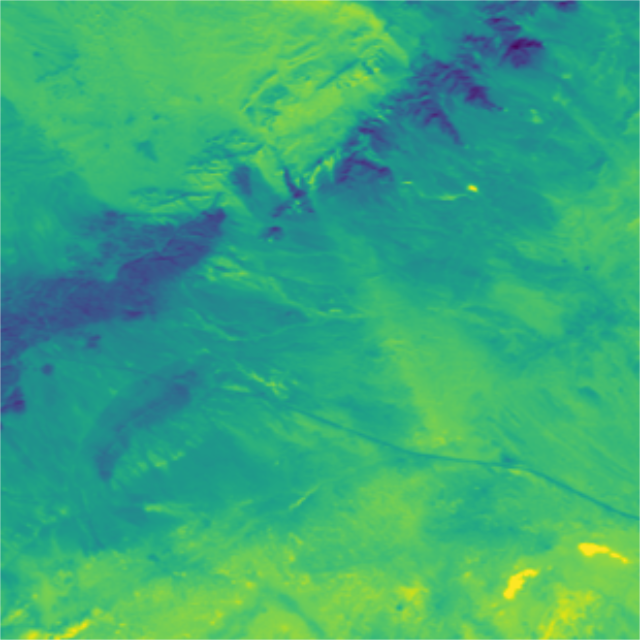
\includegraphics[width=\textwidth]{intermediate_hr}
        \caption{High--resolution}
    \end{subfigure}
    \hfill
    \centering
    \begin{subfigure}[t]{0.45\textwidth}
        \centering
        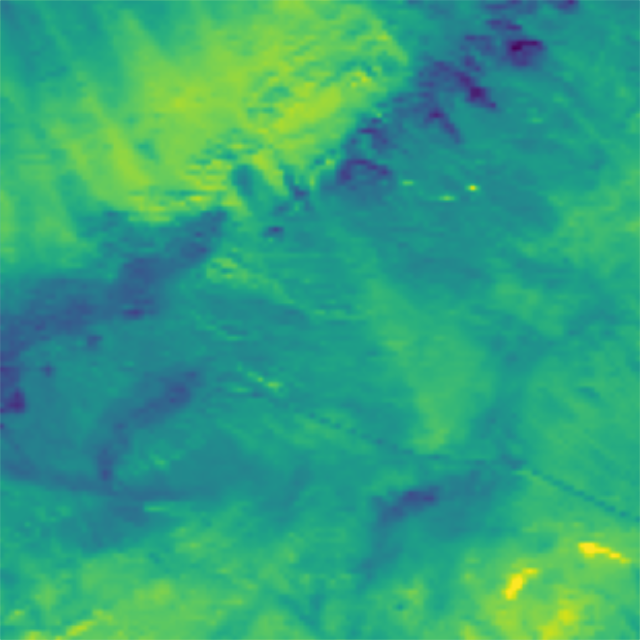
\includegraphics[width=\textwidth]{intermediate_lr}
        \caption{Low--resolution}
    \end{subfigure}
    \vskip\baselineskip
    \begin{subfigure}[t]{0.45\textwidth}
        \centering
        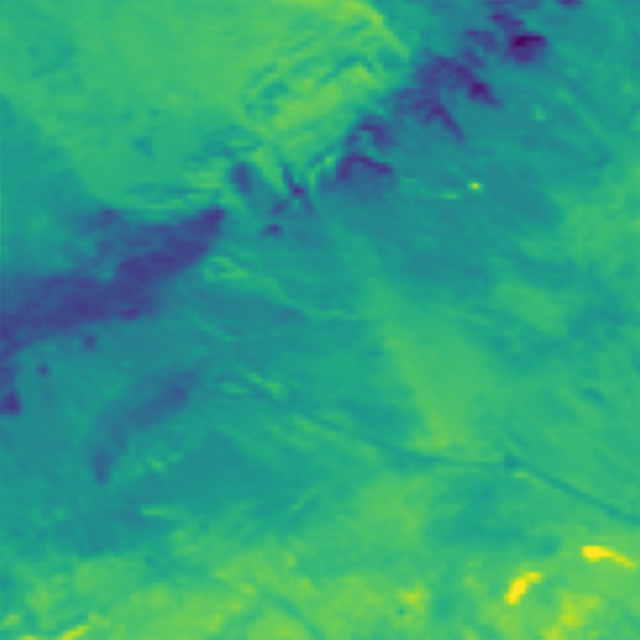
\includegraphics[width=\textwidth]{intermediate_lr_pred}
        \caption{Low--resolution augmented}
    \end{subfigure}
    \hfill
    \begin{subfigure}[t]{0.45\textwidth}
        \centering
        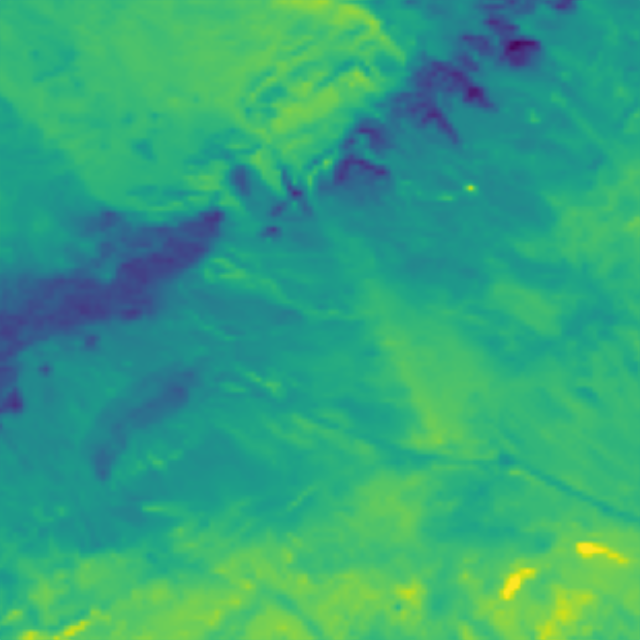
\includegraphics[width=\textwidth]{intermediate_lr_bicubic}
        \caption{Low resolution resized with bicubic}
    \end{subfigure}
    \caption{Intermediate results of evaluation on Proba--V test dataset for simple convolutional augmentation network}
    \label{fig:intermediate-results}
\end{figure}
\begin{figure}
    \begin{subfigure}[t]{0.45\textwidth}
        \centering
        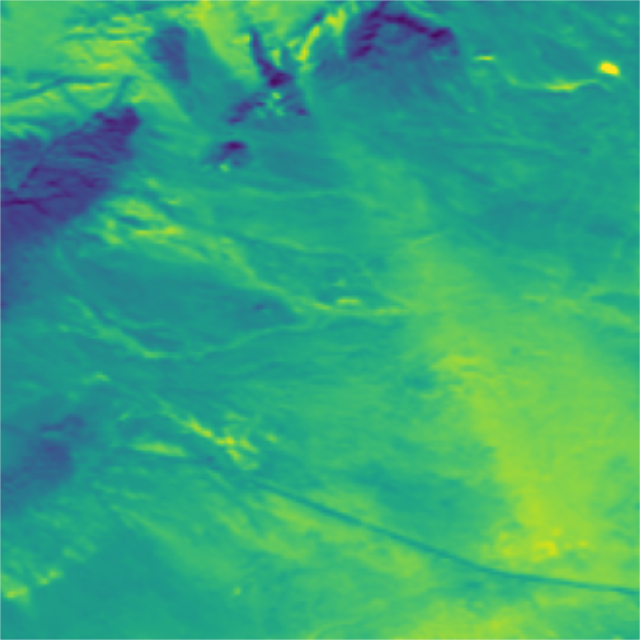
\includegraphics[width=\textwidth]{intermediate_zoomed_hr}
        \caption{High--resolution}
    \end{subfigure}
    \hfill
    \centering
    \begin{subfigure}[t]{0.45\textwidth}
        \centering
        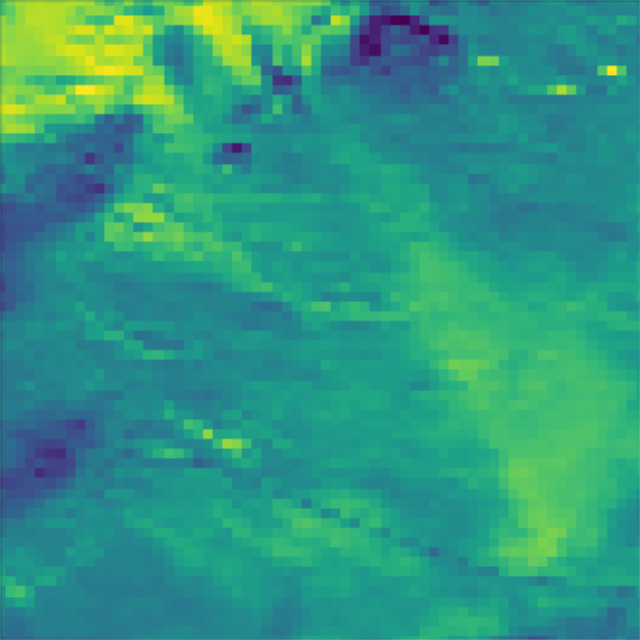
\includegraphics[width=\textwidth]{intermediate_zoomed_lr}
        \caption{Low--resolution}
    \end{subfigure}
    \vskip\baselineskip
    \begin{subfigure}[t]{0.45\textwidth}
        \centering
        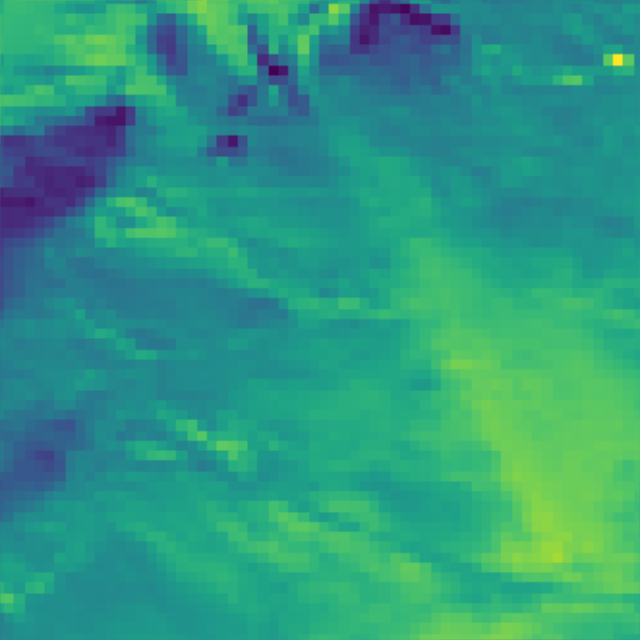
\includegraphics[width=\textwidth]{intermediate_zoomed_lr_pred}
        \caption{Low--resolution augmented}
    \end{subfigure}
    \hfill
    \begin{subfigure}[t]{0.45\textwidth}
        \centering
        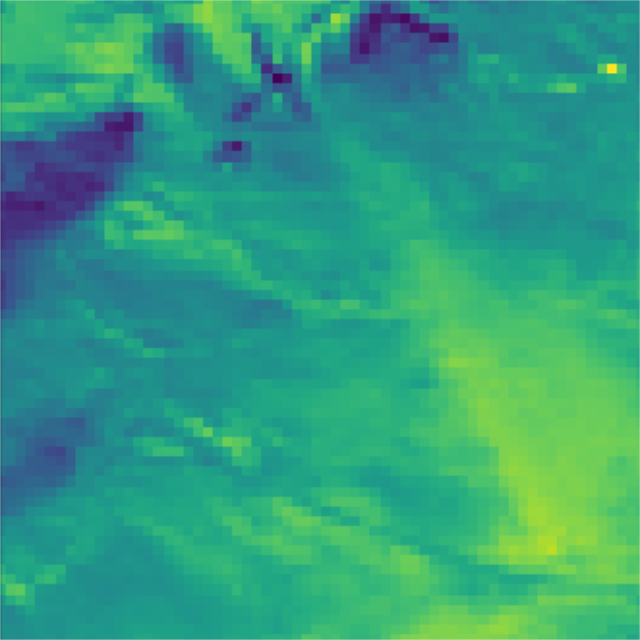
\includegraphics[width=\textwidth]{intermediate_zoomed_lr_bicubic}
        \caption{Low resolution resized with bicubic}
    \end{subfigure}
    \caption{Zoomed intermediate results of evaluation on Proba--V test dataset for simple convolutional augmentation network}
    \label{fig:intermediate-results-zoomed}
\end{figure}

The intermediate results indicate that the augmentation process works reasonably well and can be used for creating new datasets.
The numeric metrics look fairly similar for all given methods, their usefulness is to be determined during super--resolution training and evaluation.
Visual results also look well, low--resolution images resemble high--resolution ones.

\section{Implementation details}
As stated before, all networks were implemented in \textit{Python} using \textit{Tensorflow 2} library.
The built--in Keras interface offers several ways of building models; the most flexible one is called \textit{model subclassing}.
This approach enables using binary masks during training.
Model subclassing involves inheritance to implement custom training loops for Tensorflow models.
The simple convolutional and endcoder--decoder networks utilize this kind of model instantiation.
The GAN model uses a mixture of subclassing and \textit{Sequential API} which defines the model in a declarative way.
The two components of GAN---the generator and the discriminator are instantiated using the sequential approach, then they are combined into one using model subclassing.

\textit{Tensorboard} is a package accompanying Tensorflow that provides a convenient interface for training supervision.
It runs as a web server that displays a web page with the live progress of training in the form of interactive plots.
Tensorboard data is created using Keras' callbacks.
Callbacks are functions hooks called during specific steps of training.
They can provide features like previously discussed early stopping.
\textit{Model checkpoint} is another useful callback that saves the model at the end of the training epoch.
Tensorflow provides an interface for creating custom callbacks.
An inference preview mechanism on validation image at the end of each epoch was implemented as a custom callback.
This mechanism is very convenient when training the \textsc{gan} network.
Keras also enables writing custom losses and metrics.
This possibility has been used to write training losses based on PSNR and SSIM.
Both of them are based on internal Tensorflow implementations that were adjusted to serve as loss functions.